\documentclass[11pt,a4paper]{article}
%
\usepackage{graphicx}   % only required graphics package for DVI and PDF

% natbib approach
\usepackage{natbib}
\bibliographystyle{elsarticle-harv}

%\usepackage{lineno}

\usepackage[small,bf]{caption}   % allows for caption text options etc
\usepackage{booktabs}   % cool tables
\usepackage{ctable}     % allow flexible captions and footnotes for tables

% include all math symbol packages by default
\usepackage{amsmath}
\usepackage{amssymb}
\usepackage{latexsym}
%
%% do spacing
%% vital for accurate page layouts
\usepackage[margin=3cm]{geometry}

%%% change labelling of figures

% set membership slightly too large and cramped normally
\newcommand{\subin}{\, \scriptscriptstyle \in \,}

% exponentials as Roman e
% \renewcommand{\exp}{\text{e}}

% do sensible things with footnotes
\renewcommand{\thefootnote}{\fnsymbol{footnote}}

%%% option for double-spacing
%\renewcommand{\baselinestretch}{1.66}

% page-numbers at top
\pagestyle{myheadings}
%\thispagestyle{empty}
%\pagestyle{empty}

\begin{document}

\noindent {\bf {\large Consensus community detection for clustering neural data}}

\vspace{5mm}

\noindent Last updated: 20 October 2014

\vspace{5mm}

\noindent Mark Humphries
\vspace{5mm}


\tableofcontents

\vspace{0.5cm}

\section{Introduction}
Network theory provides a powerful framework for modelling the functional correlations of neurons. By representing each neuron as a node and each correlation as a weighted link, we define a functional network of cellular-level activity \citep{Humphries2011}. A key challenge in network analysis is how to divide a network into groups --- or {\em modules} --- such that the nodes in each module are densely connected with each other but weakly connected to nodes in other modules (for review see \citep{Fortunato2010,Newman2012}). This is usually termed the problem of ``community detection'', by analogy with detecting meaningful groupings in social networks. The division of our functional network into modules thus defines potential neural ensembles.

We first briefly recap our community detection algorithm from \citep{Humphries2011} (see paper supplied with the Documentation), which provides a fast, scalable approach that directly maximises a quantitative measure of modularity. We then introduce our novel algorithm for producing consensus clusterings using that community detection algorithm, which allows for highly reproducible groupings of the same data-set.

\section{Defining the functional network}
Our starting point is the weighted network matrix $\mathbf{W}$ whose entries $W_{ij}$ give the positive correlation between neurons $i$ and $j$. We emphasise that the modular-deconstruction approach to such cellular-level functional networks is highly general. The matrix $W$ can be constructed from a wide range of spike-train correlation measures, on time-scales ranging from milliseconds to seconds (as we demonstrated in \citep{Humphries2011}). For example, one could first convolve each spike-train with an exponential, Gaussian, Epanechnikov, or other kernel, then compute pairwise correlations using cosine similarity, the correlation coefficient, or other linear measure. Alternatively, one could compute the pair-wise correlations using metrics specific to spike-train structure, such as the Victor-Purpura distance \citep{Victor1996}, Lyttle-Fellous burst metric \citep{Lyttle2011} or the parameter-free ISI-distance \citep{Kreuz2007}. Modules within the functional network then quantitatively define a ``neural ensemble" independently of the specific time-scale and choice of pair-wise correlation measure.

In the example script supplied here we use a rectified correlation coefficient computed between pairs of Gaussian-convolved spike-trains at zero-lag. These choices were made as we were interested in simultaneous spiking of neurons in common phases of the overall oscillatory motor program.

\section{Community detection using spectral decomposition}
Our goal is to divide the functional network into its component modules. We seek to optimise the modularity $Q$ of this matrix, informally defined as $Q$ = \{number of links within a module\} - \{expected number of such links\}. Optimising the modularity thus requires the placement of all nodes into an unknown number of modules of unknown sizes.

To begin, we form the modularity matrix \citep{Newman2006a}
\begin{equation}
\mathbf{B} = \mathbf{W} - \mathbf{P},
\end{equation}
where $\mathbf{P}$ is a matrix encoding a suitable null model network; following \citep{Newman2006a,Humphries2011} we use the model with entries between nodes $(i,j)$ of $P_{ij} = k_i k_j / m$, where $k_i, k_j$ are the total weight of links made by nodes $i$ and $j$, and $m$ is the total weight of the network. This model gives the ensemble average of networks with the same expected distribution of weights per node as the data network, ignoring any correlation between nodes that may arise from modular structure in the data network.

Assume we are given some arbitrary assignment of all nodes $n$ to a set of $M$ modules, encoded by the $ n \times M$ binary matrix $\mathbf{S}$: each of the $M$ columns encodes the membership of that module, so that entry $S_{ij} = 1$ for node $i$ in module $j$, and is 0 otherwise. From this, we can quantitatively define the informal notion of modularity as \citep{Newman2006a}
\begin{equation}\label{eq:Q}
Q = \mathrm{Tr}(\mathbf{S}^{T}\mathbf{B}\mathbf{S}),
\end{equation}
where $\mathrm{Tr}$ indicates the matrix trace, and $^T$ is the matrix transpose.

We thus seek some assignment of nodes in $\mathbf{S}$ that maximises Equation \ref{eq:Q}. Our starting point is an eigenspectra decomposition of $\mathbf{B}$: as $\mathbf{B}$ is a centred matrix with mean of zero, the number of $p$ positive eigenvalues indicates the maximum number of detectable modules in the network \citep{Newman2006a}.

We proceed as follows \citep{Humphries2011}. The $p$ eigenvectors corresponding to all positive eigenvalues form a $p$-dimensional projection of the modularity matrix, in which entry $i$ in each eigenvector together specify the $p$-dimensional co-ordinates of node $i$. We thus cluster in this space to determine the module membership. We consider in turn each possible number of modules between $k=2$ and $p+1$ (as the first eigenvector denotes two modules, given by the sign of its entries). For each $k$, we repeat k-means clustering 100 times, using Euclidean distance. Each k-means clustering returns an assignment of each node to a module, for which we compute $Q$.

Out of all $100 \times p$ clusterings, the one that maximises $Q$ is a viable definition of the neural ensembles present in the recording. In \citep{Humphries2011} we showed how this can give insights into the evoked firing of dopaminergic neurons, and the spontaneous activity of cortex in vivo. However, the need to combine modules from across recordings presented a stern new challenge.

\section{Consensus community detection}
One distinct advantage of using modularity optimisation is that not only is it a demonstrably powerful approach to the analysis of networks \citep{Newman2006a,Newman2006b,Nadakuditi2012}, but also its limitations are very well characterised. This both allows us to interpret its output correctly, and to understand how to solve specific problems. The search space for modules is astronomically large: for $N$ neurons, the number of possible groups ranges between 1 (all neurons in one group) and $N$ (each neuron in its own group), and so the total number of group permutations is given by the Bell number for $N$; for 100 neurons, the number of possible groupings is $\sim 4.75 \times 10^{115}$. Given the astronomical size, sampling this space usually requires that the algorithms are stochastic in that each single iteration of the algorithm starts from a different initial condition (as in the k-means step from the above algorithm) and/or starts with a different initialisation of the random number generator.

Like all known benefit or cost functions for stochastic unsupervised clustering, maximising $Q$ is a NP-complete problem \citep{Brandes2006}; thus all algorithms can only be heuristic approximations to finding the solution with maximum $Q$ within this astronomical search space. Moreover, it is known that many solutions with high values of $Q$ exist, and often form plateaus around the maximum-valued solution(s) \citep{Good2010}. Consequently, each run of any good stochastic unsupervised clustering algorithm, such as the above, is likely to return good solutions that are related but different sets of modules.

In practical contexts, such variability can be undesirable. In many applications, we have a set of networks representing a set of related samples from the system under study, and we wish to combine the analyses of those networks to build a picture of the whole system. We thus would like to combine the results of community detection on each network, but this is particularly difficult to do if applying an algorithm to each network will return different good clusterings. A method for finding both a good solution and a consistent solution is needed to allow such combinations.

In this regard neural recording studies, whether cellular-level as here or at the macroscopic scale of fMRI and EEG \citep{Bullmore2009}, are particularly challenging because each data-set that defines a single network is a noisy incomplete sample from a large, relatively unknown neural system. Understanding the neural system thus requires the combination of all sampled networks. In our first application of these methods, the challenge was to define neural ensembles consistently between recordings, so that we could combine those recordings to quantitatively examine the common functional and physical properties of the {\em Aplysia} pedal ganglion (Bruno et al, in revision).

Our solution here is to use the consensus clustering approach \citep{Monti2003,Nguyen2007}. The general idea is that a stochastic clustering algorithm will return a total of $g$ clusterings, and each clustering $G$ contains some information about the most reliable partition of the data-set into groups. Lancichinetti and Fortunato \citep{Lancichinetti2012} recently introduced the use of this idea into the problem of community detection. Inspired by this, we developed a novel consensus community detection algorithm that, crucially, is parameter-free: it self-determines both the appropriate clustering and its convergence.

Our consensus algorithm is generally applicable to arbitrary networks. For our present purposes, it provides a powerful solution to the problem of generating reliable neural ensembles before comparison between and merging across recordings.

\subsection{Consensus algorithm}
Given the initial weighted network $\mathbf{W}$, we retain all $g = 100 \times p$ clusterings in set $\mathbb{G}$ produced by the above spectral clustering algorithm of modularity maximisation. We then iteratively proceed as follows:
\begin{enumerate}
    \item From set $\mathbb{G}$ remove all clusterings that have $Q \leq 0$ as these provide no information about modularity, giving set $\mathbb{G}^*$ with $g^*$ clusterings in total.
    \item Produce the {\em consensus matrix} $\mathbf{C}$: entry $C_{ij} = n_{ij} / g^*$ is the proportion of times each pair of nodes $(i,j)$ are placed in the same module.
    \item Check for convergence of the consensus matrix (see below):
        \begin{enumerate}
            \item If converged, stop; return the single clustering defined by the consensus matrix (see below)
            \item If not converged, cluster the consensus matrix using the spectral algorithm giving a new set of clusterings $\mathbb{G}$; repeat from step (1).
            \item If not converged after 50 iterations, exit with current best answer.
        \end{enumerate}
\end{enumerate}
Note that this algorithm is simple because the consensus matrix defines another weighted network that can be directly input to the spectral algorithm. Figure \ref{fig:consensus} shows this algorithm in action on one of the recordings in this paper.

\begin{figure}
\centering
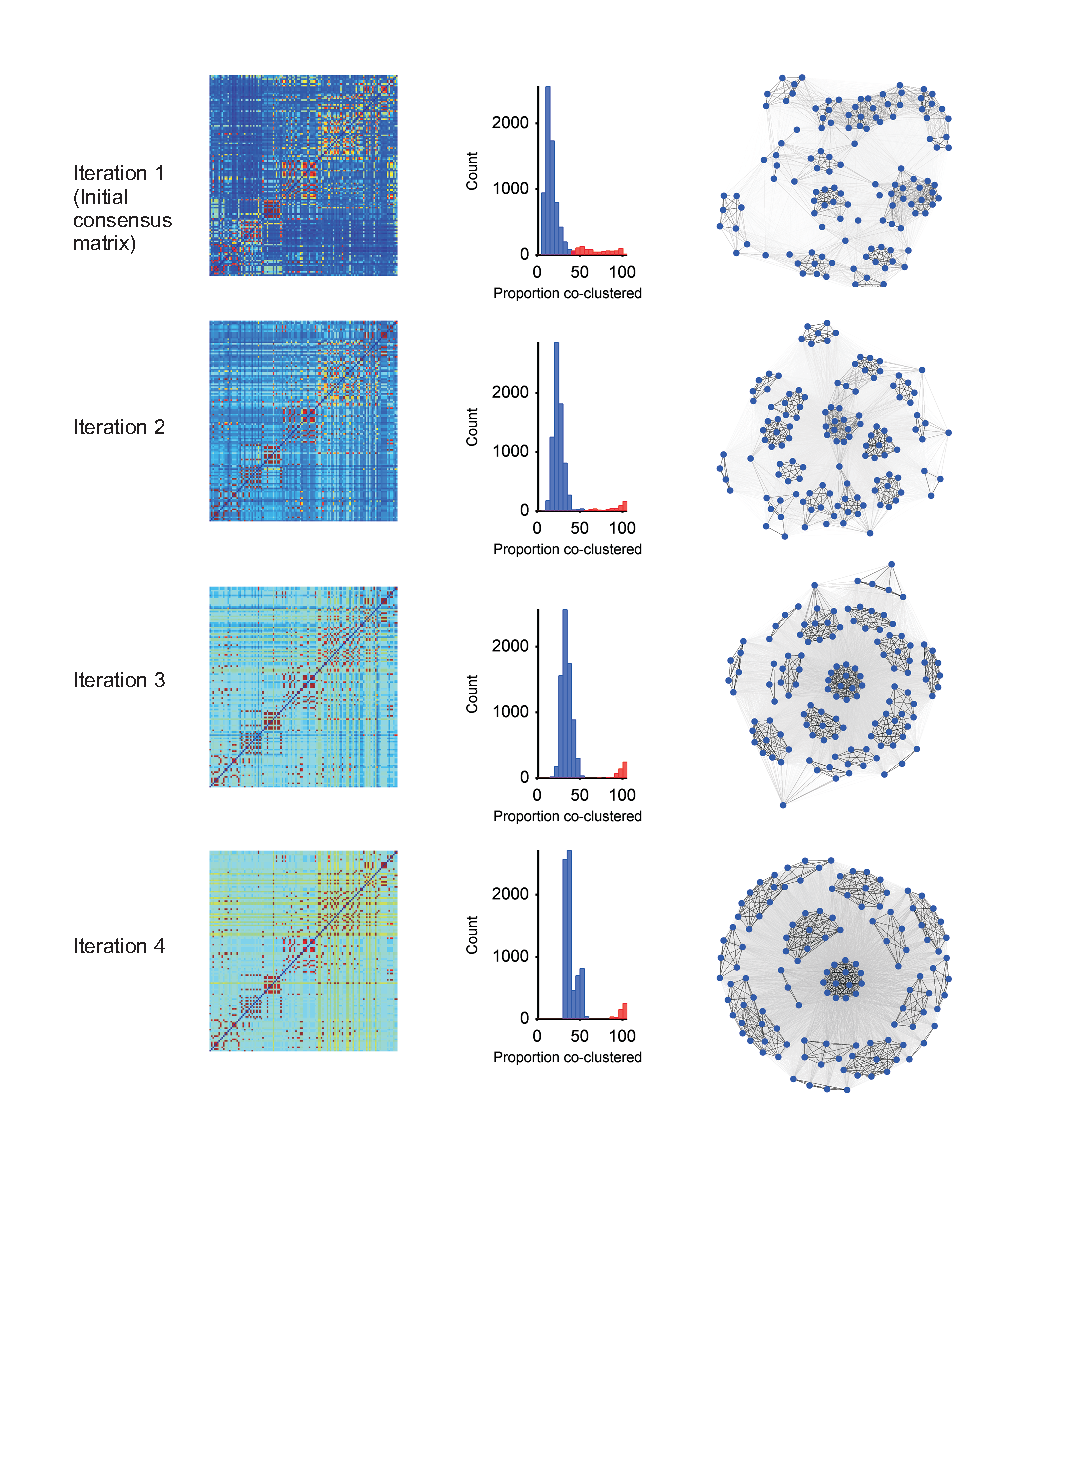
\includegraphics{Figures/SI_Figure_Consensus}
\caption{\label{fig:consensus} {\bf Example output of the consensus algorithm for community detection}. Each row shows properties of the consensus matrix $\mathbf{C}$ for one iteration of the algorithm, from the initial consensus matrix built from the clustering of the recorded data, to the final converged matrix after four iterations. The rows depict: left, the consensus matrix visualised as a pseudo-colour plot, colour intensity (blue-red) of each square coding the proportion of times that pair of nodes $(i,j)$ are placed in the same module; middle: histogram of entries in the consensus matrix, colour-coded to show the two distributions ($\mathbb{C}^{low}$,$\mathbb{C}^{high}$) found by the k-means clustering of those entries; right: network visualisation of the consensus matrix, with each link's greyscale intensity proportional to the consensus matrix entry for that pair of nodes. The network visualisation clearly shows how the increasing bimodality of the consensus matrix over the iterations corresponds to the separation of the original data-set into a single set of modules.}
\end{figure}

\subsection{Convergence}
The values of the consensus matrix will become bimodal in the presence of any detectable modular structure: the distribution around the upper mode will comprise entries corresponding to pairs of nodes consistently clustered together because of their shared membership of a common module; the distribution around the lower mode will comprise entries corresponding to pairs of nodes clustered together at random (Figure \ref{fig:consensus}). Thus, our convergence condition is that the entries of the upper distribution define a single, unique clustering of the nodes.

On each iteration, we check this criterion as follows:
\begin{itemize}
\item We cluster the entries of $\mathbf{C}$ into two groups $\mathbb{C}^{low}$ and $\mathbb{C}^{high}$ corresponding to the two modes. We used k-means with $k=2$ and initial centroid values of [0.4,0.9].
\item We then check for the presence of a single clustering in the upper distribution. We first create two lists: an empty list of assigned nodes, and a list of unassigned nodes that initially contains all nodes.
    \begin{enumerate}
        \item Picking any node at random from the unassigned list, we create a module containing that node and all other nodes with which it has a non-zero entry in $\mathbb{C}^{high}$.
        \item If any of these nodes are already in the assigned list, then the upper distribution does not define a unique clustering. We exit and continue the consensus algorithm.
        \item Otherwise these nodes are moved to the assigned list.
        \item Repeat from step (1) until either we have exited (at step 2) or all nodes are assigned.
    \end{enumerate}
\end{itemize}
Thus, if each node is assigned, then we have produced a single consensus clustering of all nodes into modules.


This convergence criterion was reliable for every recorded data-set from this study, as well as all further example networks we have tested (the catch condition to exit after 50 iterations was never reached). 

%\section{Hierarchical consensus clustering}
%The consensus clustering algorithm gives a conservative division of a network into the most strongly defined modules, and thus solves our main problem of listing the functional components of a neural circuit from large-scale recordings. However, networks often contain a hierarchical structure of module sub-divisions \citep{Clauset2008}, with each ascending level indicating weaker but meaningful groupings of the network. The consensus clustering results thus form the bottom level of a potential hierarchy. For a functional network defined by correlations between spike-train time-series, it is likely that the initially detected ensembles will themselves be variably correlated according to the presence or absence of oscillations and their relative phase of firing.
%
%In a further novel advance, we introduce hierarchical consensus clustering, which is similar in spirit to the well-known Louvain algorithm \citep{Blondel2008} for community detection. Figure \ref{fig:hierarchy} schematically illustrates the algorithm. We begin with the set of modules detected by the initial consensus clustering run. We then form a super-graph by aggregating each module into a node, and weighting the links between each node by the mean weight of the links between those modules. Applying our consensus clustering algorithm to the super-graph then potentially generates a grouping of modules. This grouping is the next level of the hierarchy. Iterations of this process recover any hierarchy present, stopping either when only two modules remain or when no modularity is present ($Q \leq 0$ for all clusterings).
%
%\begin{figure}
%\centering
%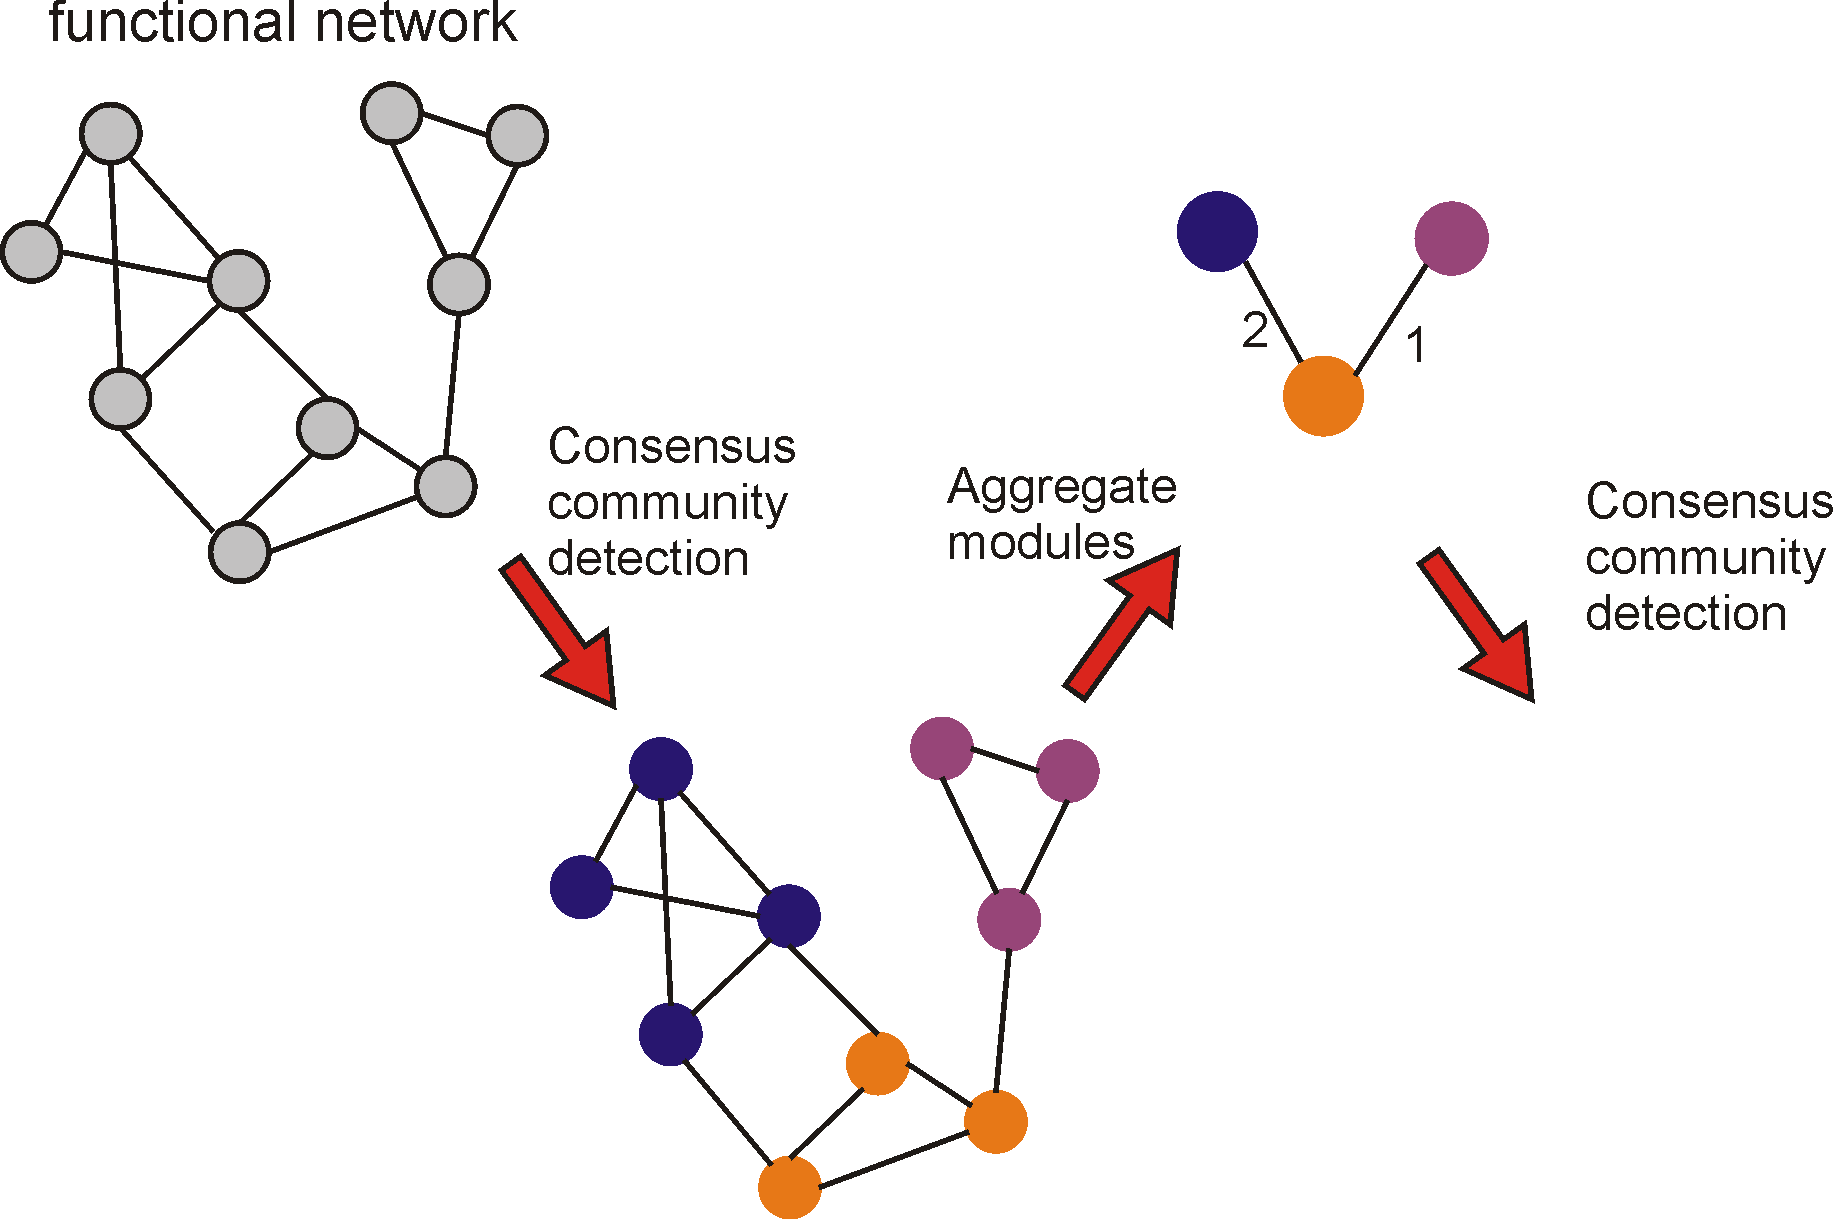
\includegraphics{Figures/SI_Figure_Hierarchy}
%\caption{\label{fig:hierarchy} {\bf Schematic of hierarchy detection algorithm}. The initial run of the consensus clustering algorithm divides the original (functional) network into modules. We then aggregate the modules into a super-graph describing the network between modules, and apply the consensus clustering algorithm to that super-graph. Any modules detected then indicate groups of modules, giving the next level of the hierarchy. This sequence can be repeated to reveal multiple levels of hierarchy, stopping either when only two modules remain or when no combination of modules is detected.}
%\end{figure}

\section{Code}
All MATLAB functions for running the consensus community detection algorithm are summarised below. Each function has extensive help text within it; here we give an overview of each function's role.

\paragraph{Main functions:}
\begin{description}
\item[consensus\_cluster\_spike\_data\_binless] The top-level function: this takes a dataset of spike-trains, and executes all steps necessary to run the algorithm on spike-train data -- convolution of each train with a function, computation of the similarity matrix from all pairs of convolved trains, and executing the consensus algorithm itself.
\item[allevsplitConTransitive] The consensus algorithm function: this takes a similarity matrix, and executes the algorithm described above. This calls the helper functions:
    \begin{description}
        \item[expectedA] Computes the null model matrix $\mathbf{P}$
        \item[spike\_train\_from\_times] Expands spike-train representation for convolution
    \end{description}
\end{description}

\paragraph{Useful functions:}
\begin{description}
\item[plot\_clusters] Visualisation of detected ensembles. Takes the spike-train data-set and a grouping of that data-set; plots the spike-trains as a raster, ordered into their detected groups
\item[sortbysimilarity] Computes various measures of each cluster's similarity, and sorts the group IDs into order of similarity
\item[MIpartitions] Computes the normalised mutual information between a pair of clusterings of the same data-set
\item[VIpartitions] Computes the variational information between a pair of clusterings of the same data-set
\end{description}

\paragraph{The toolbox is used by top-level scripts:}
\begin{description}
\item[Consensus\_Cluster\_Dataset] uses the toolbox to detect the ensembles present in each recordings in the supplied data-set
% \item[Batch\_hierarachy] runs the hierarchical version of the algorithm, given the initial clustering of each data-set. This script can be easily modified to run the hierarchical clustering on an arbitrary data-set.
\end{description}


\bibliography{CCD_refs} % bibliography file
\end{document}
